\documentclass{article}
\usepackage{amsmath}
\usepackage{braket}
\usepackage{amssymb}
\usepackage{hyperref}
\usepackage{booktabs}
\usepackage{graphicx}
\newcommand{\bfit}[1]{\textit{\textbf{#1}}}
\begin{document}
\textbf{\Large Chapter 11\\
Electron Spin Qubit in Semiconductor-Implementation, Initialization, and Readout}
\\\\\\
\textbf{\large 11.1 Introduction}\\\\
We have learned how to rotate an electron spin state using external magentic fields.
We have been assuming that the electron floats in space. In reality, it will interaction
with matters and we need to decide how to set the electron in place. We will use an electron
in silicon and illustrate how to achieve the five \textbf{DiVincenzo's criteria}
mentioned in Sect. 1.3. In this chapter, we will discuss silicon spin qubit
initialization and readout (measurement). In the next chapter, we will discuss the
implementation of 1-qubit and 1-qubit gates.\\\\
\bfit{\large 11.1.1 Learning Outcomes}\\\\
Understand why silicon qubit has the portential to enable large-scale intergration of qubits
in qunatum computers; be able to describe how to implementation quantum dot in 
a transistor; be able to describe why silicon qubit is a good qubit; be able to describe
how to initialized and measure silicon qubits.\\\\
\bfit{\large 11.1.2 Teaching Videos}\\\\
$\bullet$ Search for Ch11 in this playlist

- \url{https://tinyurl.com/3yhze3jn}\\\\
$\bullet$ Other videos

- \url{https://youtu.be/qwye4V0QXAc}

- \url{https://youtu.be/oL9f-vRcVzc}

- \url{https://youtu.be/0jVw4xICV10}\\\\\\
\textbf{\large 11.2 Why Silicon?}\\\\
At the moment of writing, the decoherence time of a qubit in most available
architechture is not long enough. Although they are long enough for maby gate
operations, there are still fininte errors due to interactions with the environment and
due to errors from gate operations (see Chap.25). As a result, quantum computing
is unreliable because most quantum computing algorithms rely on interference
and  interference fails even with tiny errors (e.g., [1]). The qubit we have been
discussing is called the \textbf{physical qubit}. In order to achieve \textbf{fault-tolerant quantum
computing}, we need to use special algorithms and multiple physical qubits to create
an error-free \textbf{logical qubit} (e.g., [2]). However, it is expected that each error-free
logical qubit will consist of 100-1000 physical qubits.

At the same time, many quantum algorithms are expected to outperform classical operations
only when the proble size is large enough. For example, it is expected that Shor's 
algorithm is only useful for a problem that needs more than 1000 \textit{logical}
qubits. Therefore, a quantum computer with 100000 to 1 million \textit{physical} qubits
is necessary to achieve practical \textbf{quantum supremacy}.

In Figs. 1.1 and 1.3, we showed that a quantum computer is just a group of
passive qubits controlled by classical electronics. If there are 1 million qubits,
how are we going to control them? In the superconducting case, without a careful architechture
design, this seems to be impossible (Fig. 1.3). Therefore, building larga-scale quantum computers using
semiconductor platforms is a natural choice. This is  especially true for the silicone platform 
as it has been proved that it can integrate more than 10 billion transistors in a few $cm^2$ and we can
harness decades of engineering experience in the silicon semiconductor industry.

Since electron spin qubits in \textbf{quantum dots} built on semiconductor platforms are small, it is
possible to integrate millions of qubits on a silicon chip. Moreover,
it is also possible to integrate the control electonics on the same chip due to
the mature technology. That means the control electronics (see Chap.23) such as low-noise
amplifiers (LNAs), analog-to-digital converters (ADCs), digital-to-analog converters (DACs),
filters, and even signal generators and processing units can be integrated
on the same platform. Readers are encourgaed to take a look at Fig.1 in [3] to see one
of the possible integration schemes.

It should also be noted that when the control electronics are near the qubits and cooled to 4.2$K$ or
below, the \textbf{throughput} will be increased and the noise will be reduced.

Ideally, if electron spin qubit can operate at 4.2K, it can be integrated on the same
chip as the control electornics and achieved minimal latency. Figure 11.1 shows an ideal 
integrated platofrm of silicon qubits and their control electronics.\\

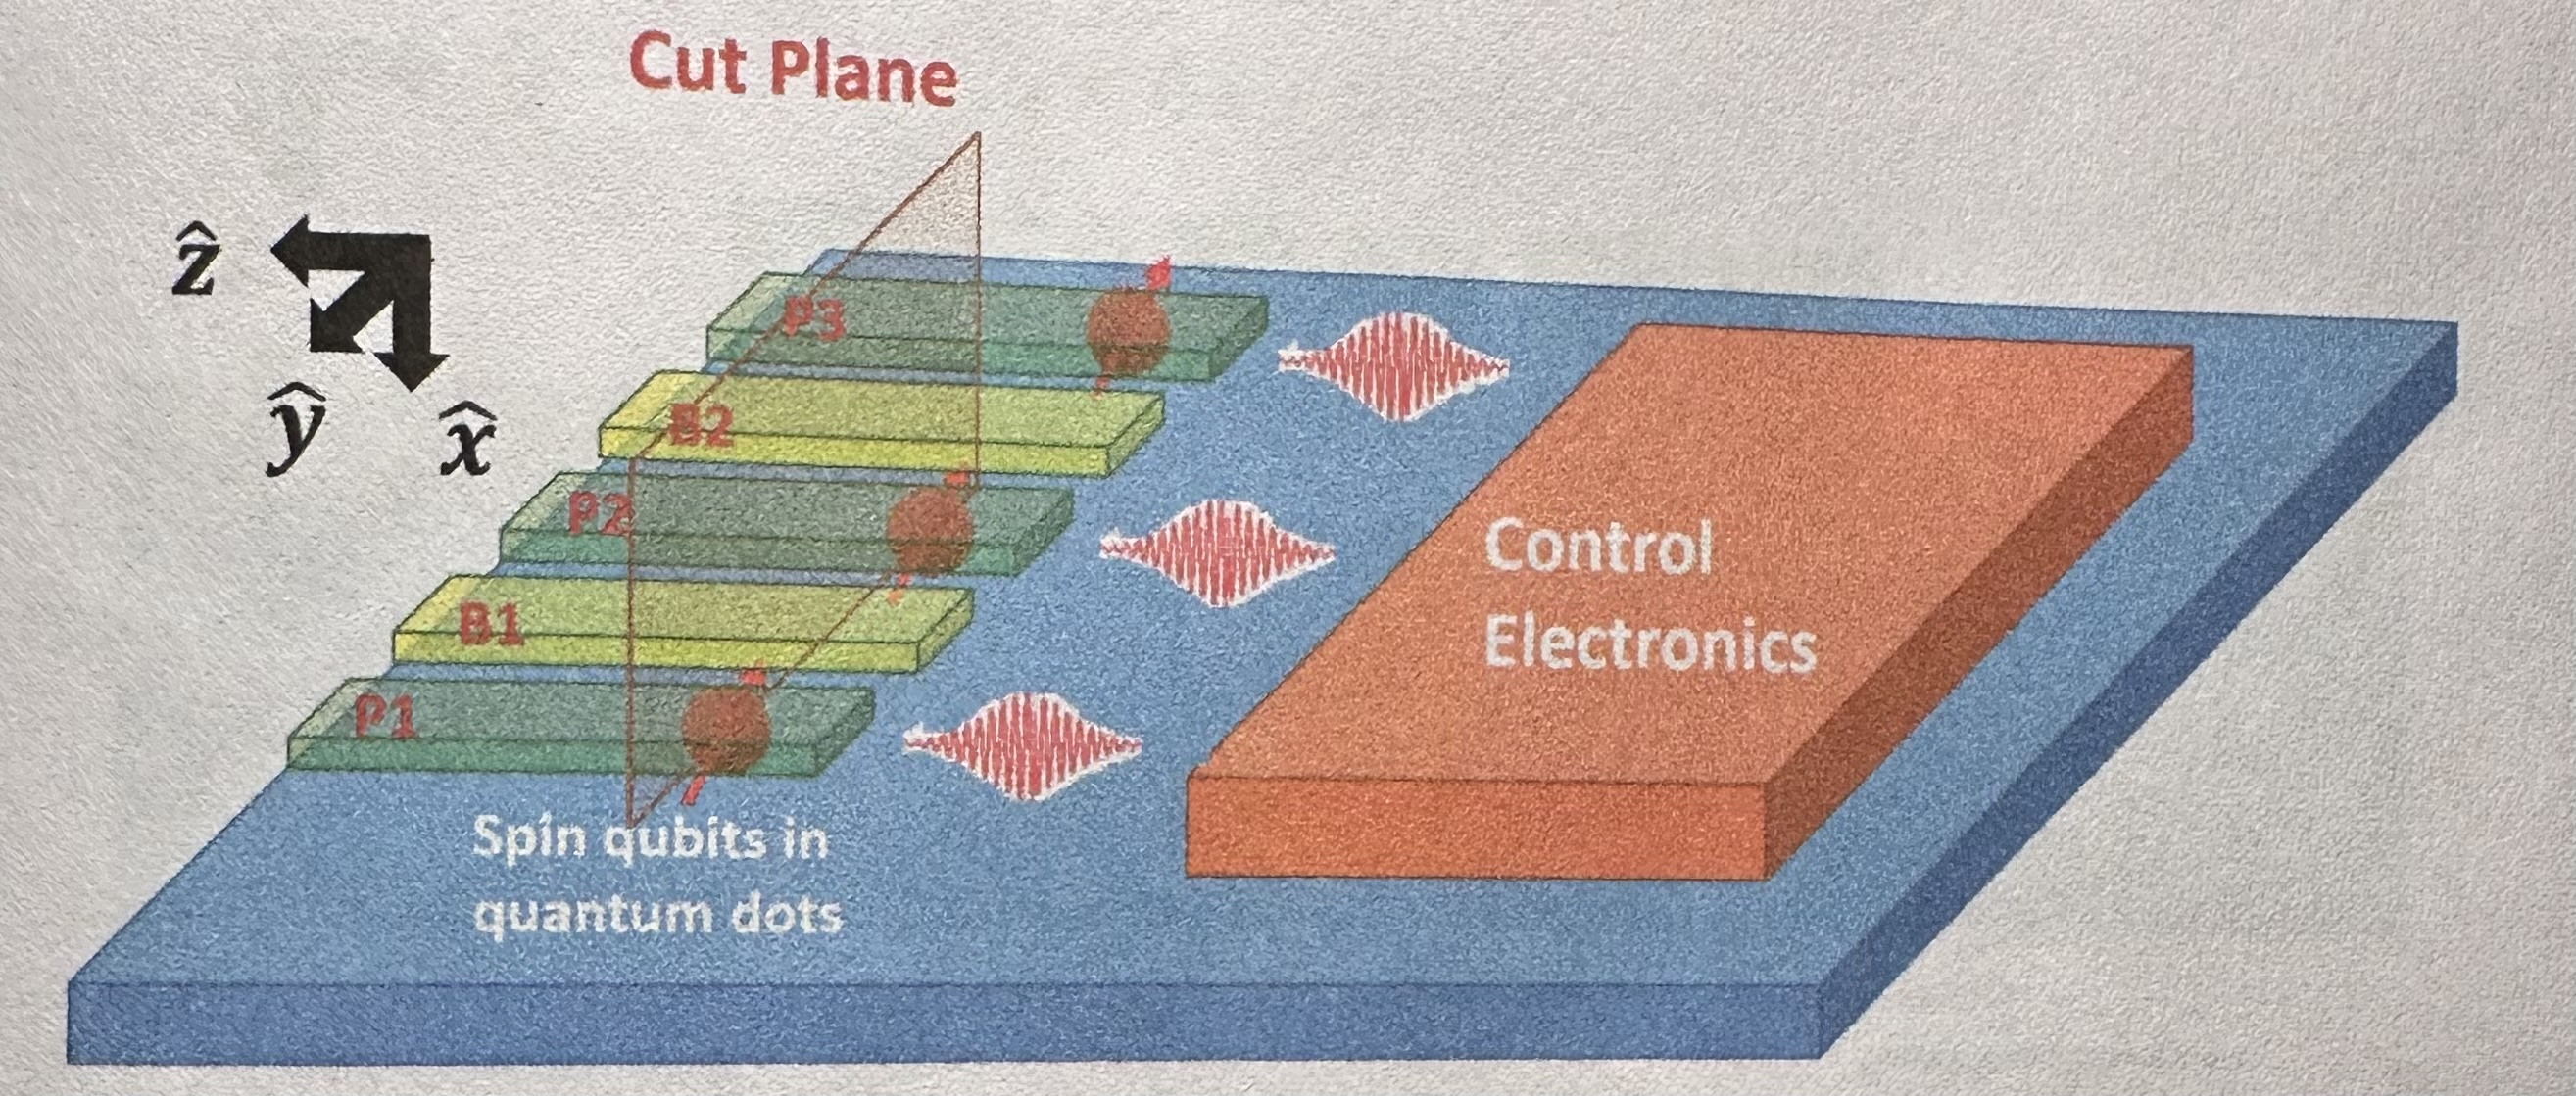
\includegraphics[scale=0.5]{Fig.11.1.jpeg}\\
\textbf{Fig. 11.1} In an \textit{ideal} and highly integrated case, silicon spin qubits are integrated on the same silicon
chip with the control electronics operating at 4.2$K$. This has minimal latency. The plunger gates
($P1, P2, P3$) and barrier gates ($B1, B2$) are shown. The plunger gates are used to form 
lateral barriers for the quantum dots. Only $\hat{y}$-direction confinement is shown here. \textit{Note that
this is a simplified shcematic. It is necessary to confine the charge also in the $\hat{z}$ direction to form
a quantum dot}. The cut plane is shown in Fig. 11.2 \\\\\\
\textbf{\large 11.3 Spin Qubits in Quantum Dots}\\\\
A common way to hold an electron carrying the spin qubit is to put it in a \textit{quantum dot}.
A quantum dot is named so because it is a tiny space in which quantum confinement becomes significant.
The enrgy of the electron becomes discretized like in an atom (which is a quantum dot also and electrons 
can only occupy discrete orbitals). More importantly, due to its small size, it has a very small capacitance. 
In order to add an additional electron to it, a large \textbf{charging energy} is required. This is because
the energy of a capacitor is given by,
\begin{equation}\label{eq 11.1}
    E=\frac{1}{2}CV^2=\frac{Q^2}{2C}, \tag{11.1}
\end{equation}
where C, V, and Q are the capacitance of the dot, the voltage across the dot,
and the charge in the dot, respectively. With a small $C$ for the Same $Q$, to add one more
charge, the energy of the whole system, $E$, increase a lot, and, thus, one can add or remove 
an individual electron to or from the dot \textit{precisely} through and electrical method.
If the energy is not enough to add an electron into the quantum dots, it is called \textbf{Coulomb blockade}
which means the charge insdie the dot is blocking the addition of another charge due to the large charging
energy.

Of course, $E$ needs to be compared to the thermal energy, $kT$, where $k$ is the Boltzmann
constant. We still need to cool the system to cryogenic temperature so that $E$ is large
compared to $kT$ to obeserve the quantum effects.

Figure 11.2 shows the cross section along a qubit array (e.g., [4]). It is similar to a typical
metal-oxide-semiconductor (MOS) transistor or capacitor. It has gates on top formed by either metal or heavily doped polycrystalline silicon.\\

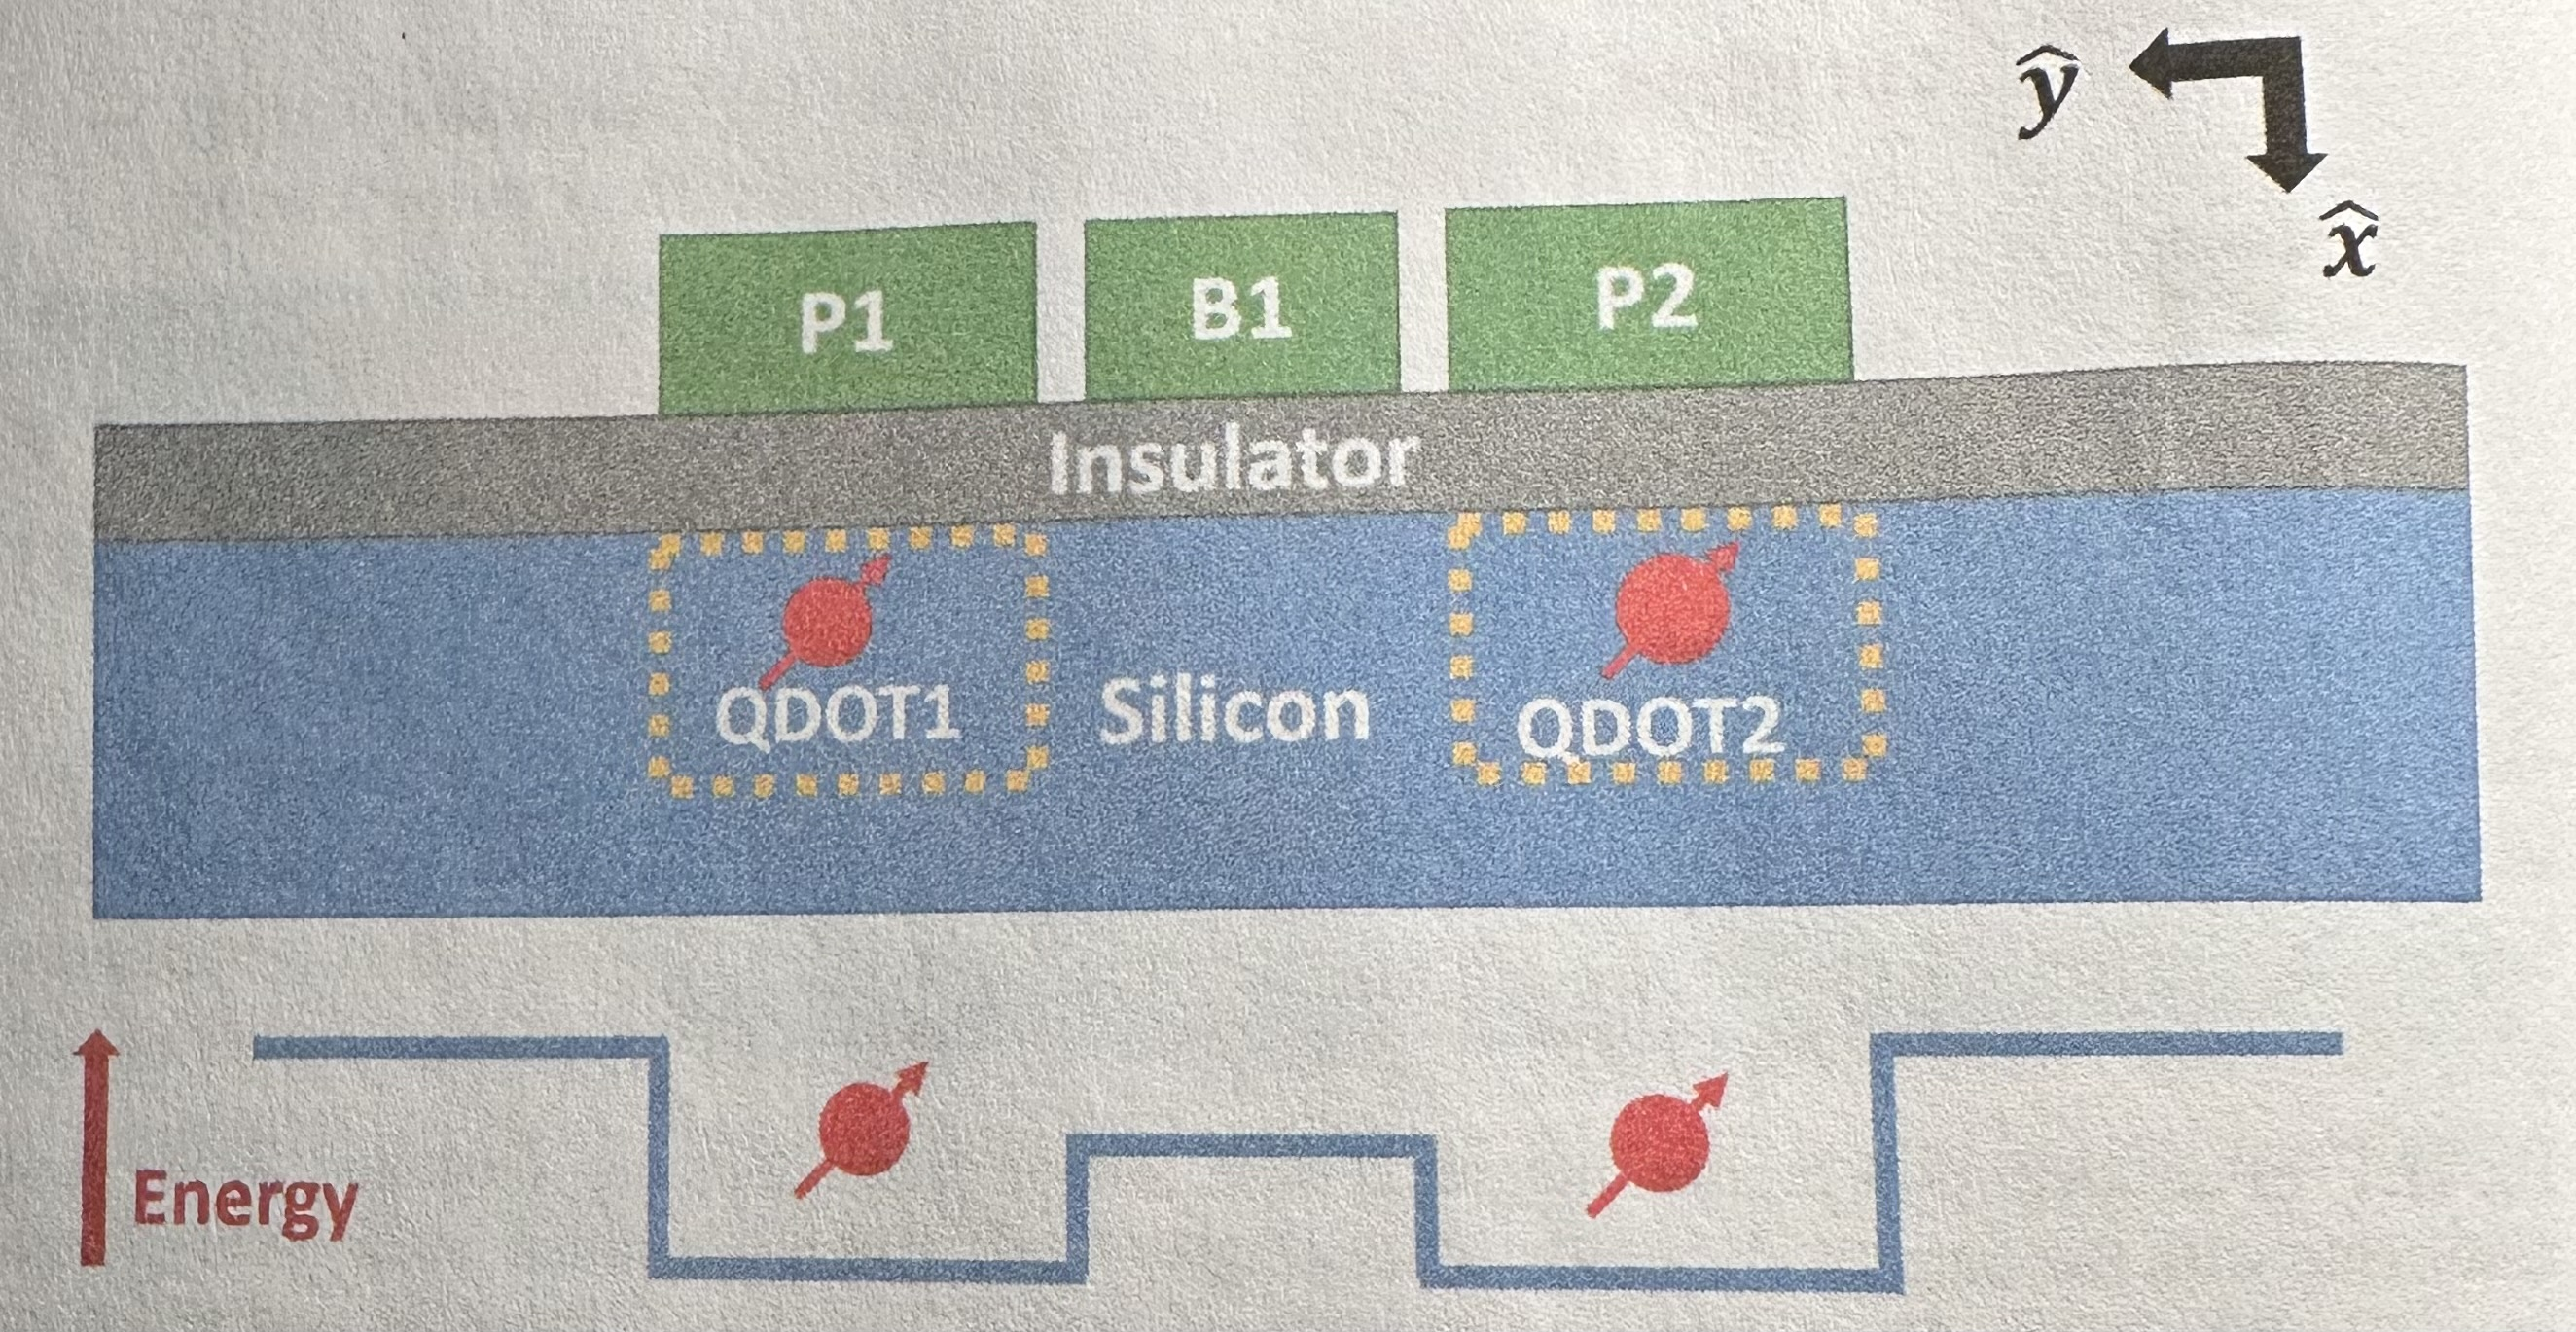
\includegraphics[scale=0.45]{Fig.11.2.jpeg}\\
\textbf{Fig. 11.2} Cut plane of Fig. 11.1 Top: Only two plunger gates and one barrier gate are shown for clarity.
Note the implementation of the vertical, $\hat{x}$-direction, confinement is not shown. Bottom: The elctron energy profile\\\\
It is capacitively coupled to the substrate (e.g., silicon) through an insulator (e.g., oxide in silicon technology).
The plunger gates, $P$1 and $P$2, are used to deplete the electron underneath and form a 
confinement potential in the vertical direction ($\hat{x}$). The barrier gate ($B$1) is used to control the potential between the plunger gates
to allow electrons to transfer or tunnel to another quantum dot by changing the barrier height.
This is a 2D corss section. In reality, the confinement should occur in the $\hat{z}$ direction also to form a quantum dot.
The drawing is simplified and did not consider this. Readers can refer to [4] to see a realistic layout. The quantum dots are formed under the plunger
gates and the lectrons arrying the qubits reside there.

Besides silicon platforms, spin qubit has also been realized in other materials, such as AlGaAs/GaAs heterostructure, 
where AlGaAs is used as the insulator as it has a wide bandgap and GaAs is the substrate (e.g., [5]).
The advantage of using the AlGaAs/GaAs system is that it has a very perfect interface that can enhance the decoherence time.
However, it is not a s scalable as the silicon platform.\\\\\\
\textbf{\large 11.4 Silicon Spin Qubit}\\\\
\textbf{Silicon spin qubit} is commonly referred to as spin qubit implemented on a silicon platform.
Most of the time, it refers to the electron or hole spin qubits. Usually, \textit{it has nothing to do
with the silicon atom itself}. In this chapter, we only look at electron spin qubits. Hole spin qubits can proide some
physics that electron spin qubits do not have [6]. For example, it has a strong \textbf{spin-orbit (SO coupling)} which allows
it to be manipulated by electrostatic (instead of magnetic field) directly. Of course, it also means
that it is more susceptible to decoherence time degradation due to the charges in the environment which are abundant.\\

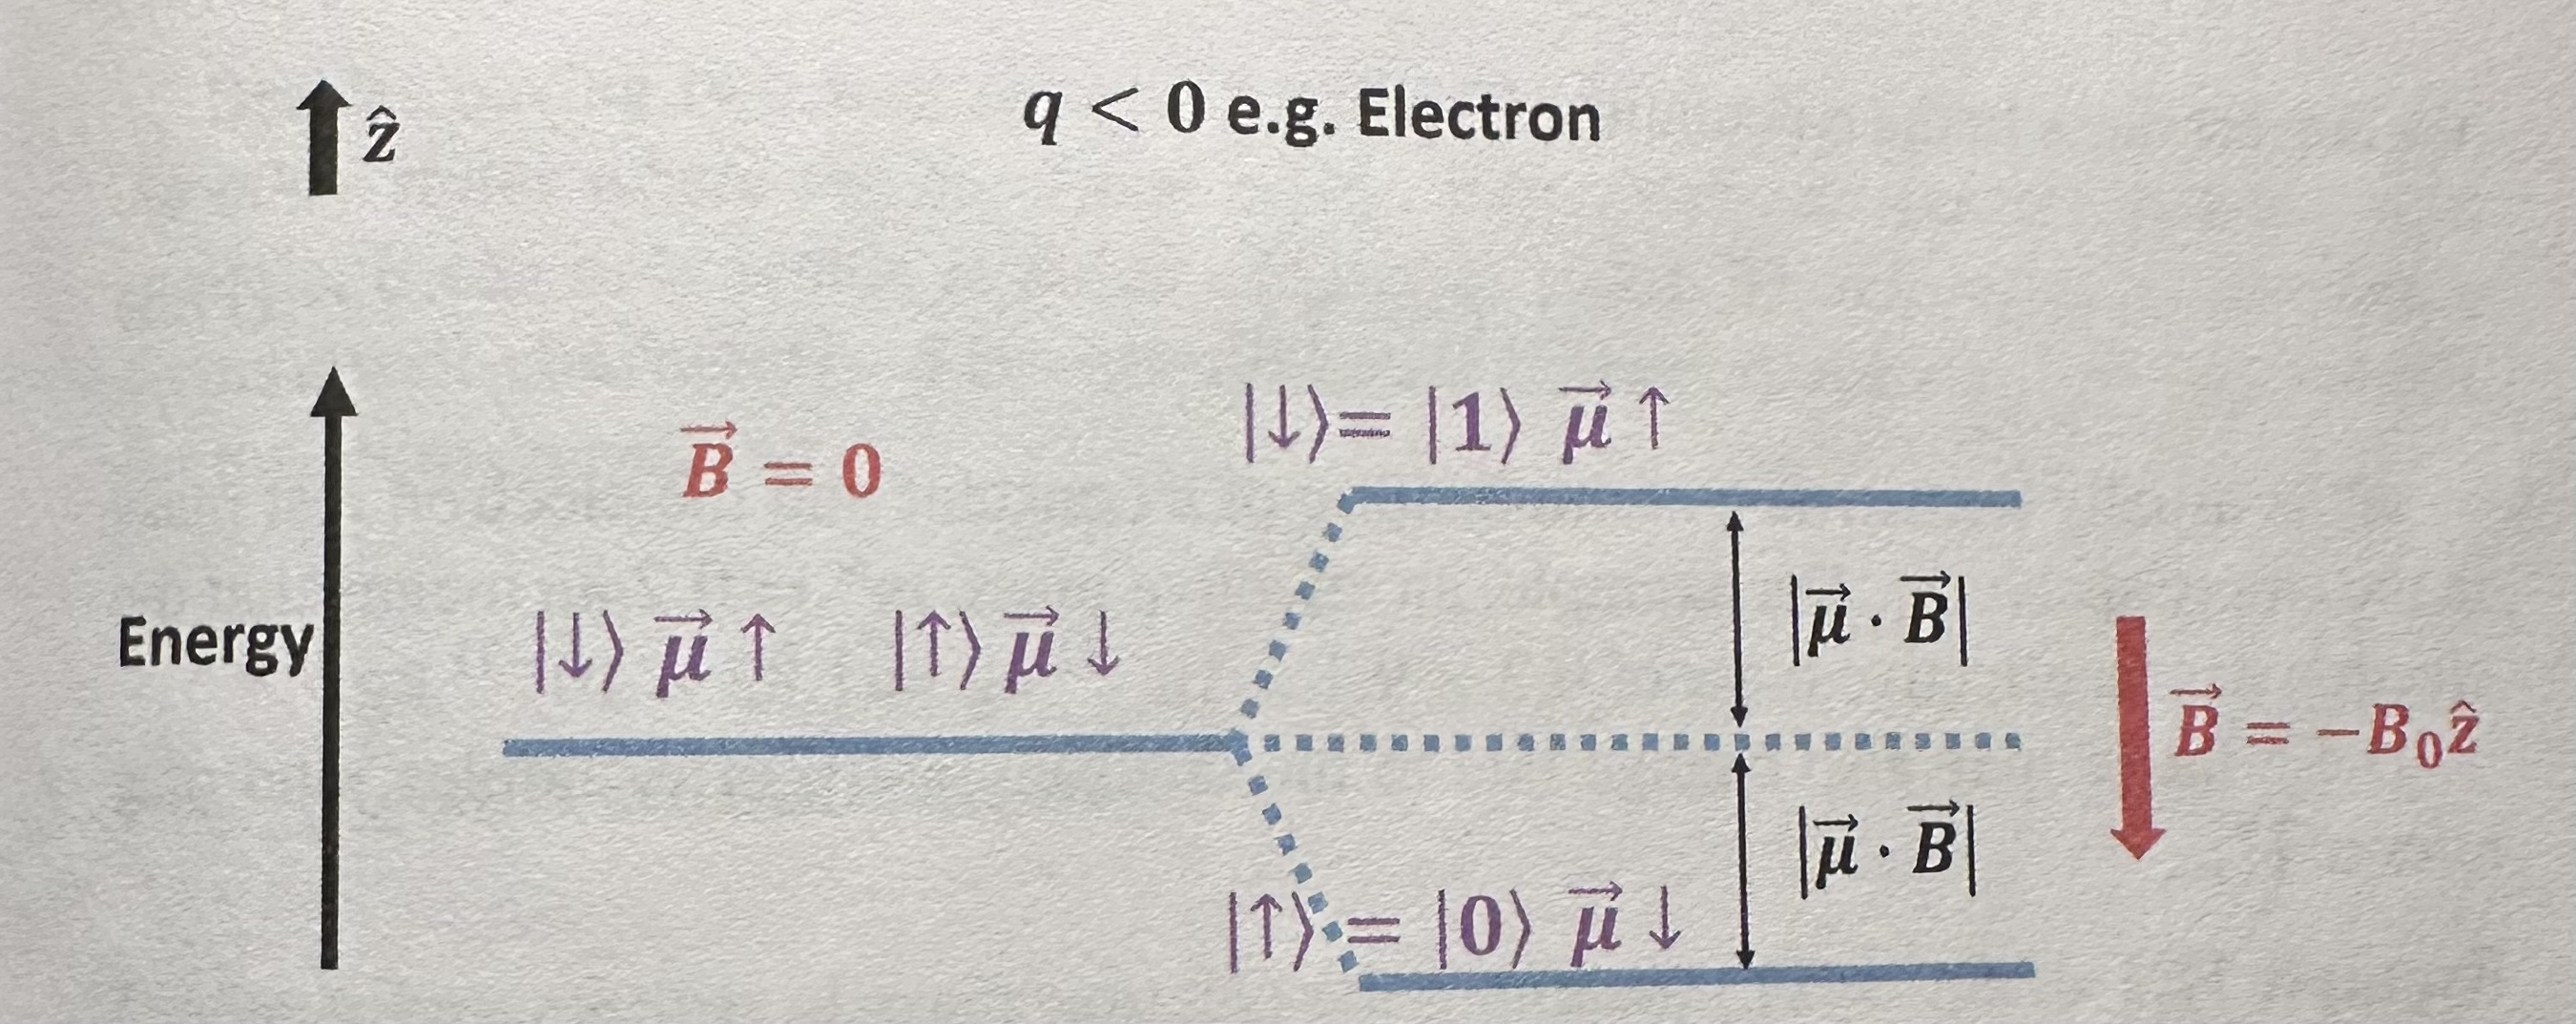
\includegraphics[scale=0.45]{Fig.11.3.jpeg}\\
\textbf{Fig. 11.3} Energy of a negatively charged particel with spin under zero (left) or a finite external
magnetic field (right). This is similar to Fig. 7.4 but with the external magenetic field pointing in an opposite direaction

Firstly, we need to encode the $\ket{0}$ and $\ket{1}$ states. This is to fulfill one of 
DiVincenzo's criteria: "A scalable physical system with well-characterized qubit." As discussed 
in the previous section, the silicon platform is probably the most scalable one.
As for "well-characterized qubit," we just need to apply a vertical magentic field
to create an energy splittingn as shown in Fig. 11.3. This is also called the \textbf{Zeeman splitting}.
The physics has been discussed in the previous chapters. Here we review the important concepts and equations.

When there is no external magnetic field, the $\ket{0}$ and $\ket{1}$ states have the same
(\textbf{degenerated}). When an external DC magnetic field is applied, the one with a 
magnetic moment parallel (anti-parallel) to the magnetic field will acquire a  lower
(higher) evergy (Eq. (7.10)). Since an electron has a negative charge, it means 
the electron with spin parallel (anti-parallel) to the magnetic field will acquire a
\textit{higher (lower)} energy (Eq.(7.9)). In Fig. 11.3, as the magnetic field points down,
the spin-down (spin-up) electron has a higher (lower) energy. The energy differences
between the two states are given by
\begin{align*}\label{eq 11.2}
    \varDelta&=2|\vec{B}\cdot\vec{\mu}|,\\
    &=2|B_0\gamma S|,\\
    &=2|B_0\gamma\hbar/2|,\\
    &=\hbar\omega_L,\tag{11.2}
\end{align*}
where we have used Eqs. (7.8), (7.10), and (8.11). It is important to recall that the gyromagnetic
ratio depends on the g-factor and also the effective electron mass, $m^*$.
In silicon, the effective mass can change substantially. We need to make sure we use
the correct mass in the calculation. Therefore,
\begin{equation}\label{eq 11.3}
    \gamma=\frac{ge}{2m^*}. \tag{11.3}
\end{equation}

$m^*$ is usually written as a muliplication of a constant and the electron rest mass in the
empty space, $m_0$. For example, an effective mass, $m^*=0.2m_0$ means that the electron has an
effective mass of $0.2\times9.1\times10^{-31}\text{kg}=1.82\times10^{-31}\text{kg}$.

The g-factor may also change due to the environment. For examples, one may refer to [7].\\\\
\textbf{Example 11.1} If $B_0=1T$, assuming the electron mass is still $m_0$ and $g=-2$, find the
energy difference between $\ket{0}$ and $\ket{1}$

Using Eq.(\ref{eq 11.2}),
\begin{align*}
    \varDelta&=2|B_0\gamma\frac{\hbar}{2}|,\\
    &=2|B_0\frac{ge}{2m}\frac{\hbar}{2}|,\\
    &=2\times1T\times\frac{2\times1.6\times10^{-19}C}{2\times9.1\times10^{-31}\text{kg}}\times
    \frac{6.625\times10^{-34}J\cdot s}{2\times2\times3.14},\\
    &=1.855\times10^{-23}J,\\
    &=116\mu eV.
\end{align*}

Note that we have converted the energy in $joule\, (J)$ to $electron-volt\, (eV)$
by using the definition (i.e., by dividing by $1.6 \times 10^{-19}C$). As a reminder, 
$1\, \mu eV=10^{-3}\, meV=10^{-6}\, eV$.

Is this a qubit with \textit{well-separated energy levels}? That depends on the operating temperature.
\\\\
\textbf{Example 11.2} What is the thermal energy at 10 mK? How does it compare to the qubit
energy in the previous example?

The thermal energy is given by $kT$, where $k$ is the Boltzmann constant which is
$1.380649\times10^{-23}$J/K and $T$ is the temperature. Therefore, the thermal energy is,
\begin{align*}\label{eq 11.4}
    kT&=1.380649\times10^{-23}\text{J/K}\times10\times10^{-3}\text{K},\\
    &=1.38\times10^{-25}J,\\
    &=0.86\mu eV.\tag{11.4}
\end{align*}

The qubit energy separation is at least 100 times larger thatn the thermal energy.
Therefore, the qubit states are well-defined. \hfill $\blacksquare$

Besides having two well-sepearted states, \textit{we also need to make sure there are no
other states where the qubit can reside}. Fortunately, an electron is a half-spin particle.
It can only reside at either $\ket{0}$ or $\ket{1}$ states. Therefore, the electron spin forms
a \textbf{well-characterized two-dimensional Hilbert space} which is very suitable for quantum computing.\\\\
\textbf{\large 11.5 Qubit Initialization}\\\\
DiVincenzo's criteria also require that an architecture should have "the ability to
intialize the state of the qubits to a simple fiducial state." For silicon spin qubit, the ground
state is $\ket{0}=\ket{\uparrow}$ if it is set up as in Fig. 11.3. To initialize a qubit, it means to make
sure the qubit is at its ground state, $\ket{0}=\ket{\uparrow}$.

We will discuss three methods to initialize a qubit.\\\\\\
\bfit{\large 11.5.1 Thermalization}\\\\
\textbf{Thermalization} is a natural and common way in all quantum computing architechtures to perform
qubit initialization. What it means is that we will let the qubit sit for a long time (e.g., 10 times of
$T_1$, which is one of the decoherence times of a qubit and will be discussed in Chap. 25).
If the qubit is already at its ground state, it will stay at the ground state. But if the qubit is at an
excited state ($\ket{1}$ or $\ket{\downarrow}$ in Fig. 11.3), due to the interaction with the environment,
it will lose its energy eventually and flip to the ground state.

Here we see the dilemma, We want to have a long decoherence time as requested by the requirement
"long relevant decoherence times" in DiVincenzo's criteria. We also want to have a short $T_1$ times
so that it can decay fast during initialization. After each unit of $T_1$, only $1-e^{-1}$ of the population
(or probability) will decay to $\ket{0}$ from $\ket{1}$. To make sure the qubit has decayed to $\ket{0}$,
we need to wait for$10T_1$. A silicon qubit may have a $T_1$ as much as 100 ms. That means we need to wait for
1$s$ in each initialization. This is considered long and can slow down quantum computing algorithms. Therefore,
this is not a desirable initialization method.\\\\\\
\bfit{\large 11.5.2 State Filtering Through Tunneling}\\\\
We may also try to filter and get rid of electrons in state $\ket{1}$ through electrical
operations to achieve the initialization purpose. This is mentioned in [8] for another purpose
but we can hijack it to perform initialization. \textbf{I have not seen people using this for initialization}. \textbf{But I think this is instructive and we can further discuss its pros and cons}.
It also prepares us for spin-to-charge conversion for readout in the following section.\\

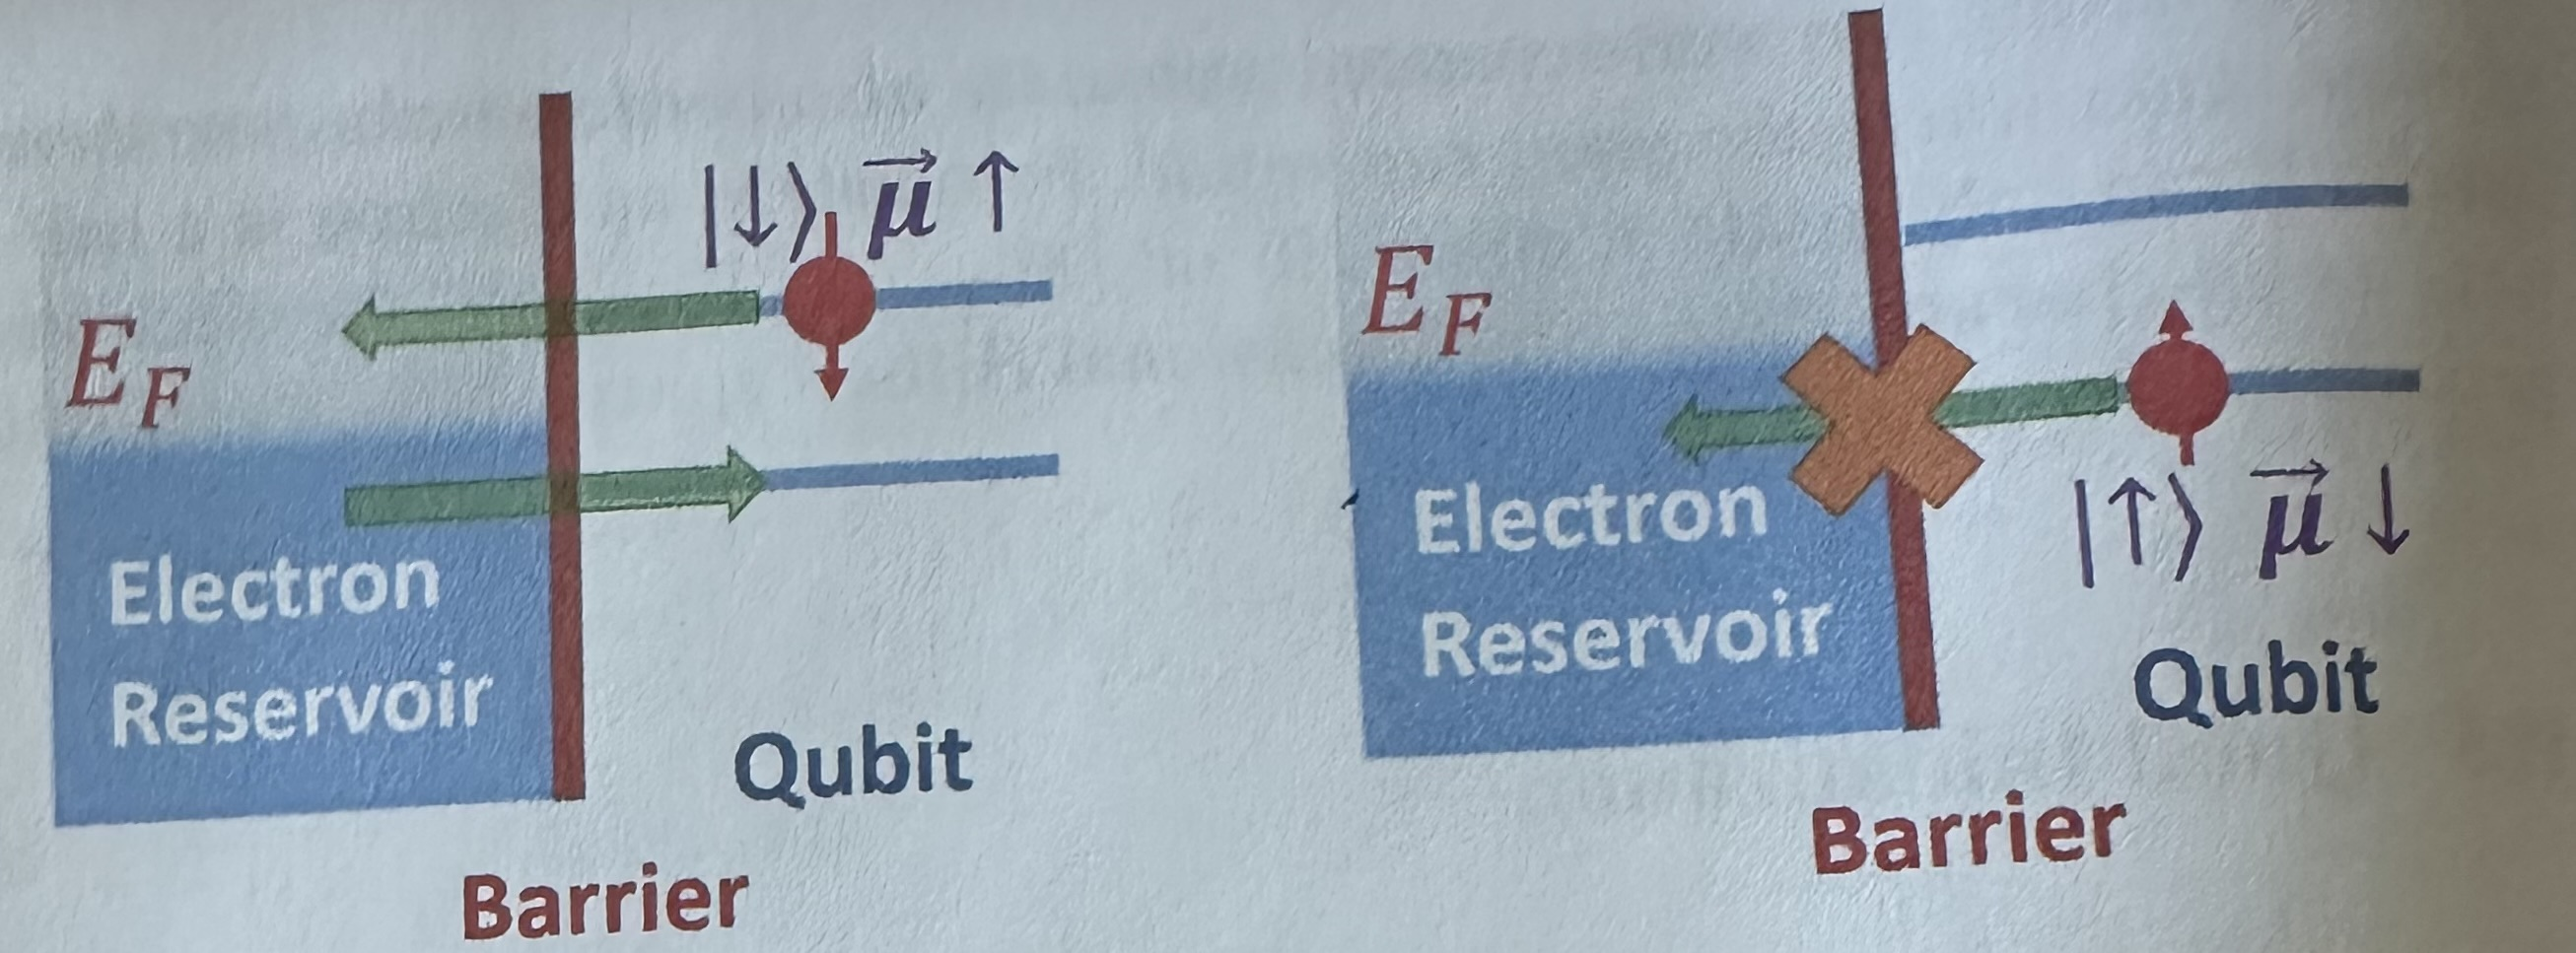
\includegraphics[scale=0.45]{Fig.11.4.jpeg}\\
\textbf{Fig. 11.4} Using state filtering to achieve initialization. The electron carrying the qubit is allowed
to tunnel into an electron reservoir. The potential of the qubit is set up such that the excited state is above
the Fermi level ($E_F$) of the reservoir and the ground state is below. On the left,
if the electron is at its excited state, it can tunnerl into the reservoir as there are empty states.
And the electron from the reservoir can then tunnel into the ground state. On the right, since the electron has
a lower energy than the Fermi level, the corresponding state is filled and it cannot tunnel\\

Figure 11.4 shows the scheme. We can make the qubit next to an electron reservoir such as metal. It is known
that in metal, there is a special energy level called the \textbf{Fermi level}, $E_F$. Above $E_F$, there is no electron, and below $E_F$, the states
are filled with electrons. What I am saying is a simplification because the states are filled by 
following the so-called Fermi-Dirac distribution (see also Eq. (16.1) and the discussions). However, the picture
is fairly accurate at very low temperatures, which is the case for most quantum computers
(see Example 11.2).

The electron carrying the qubit is separated from the metal by an insulating barrier.
Therefore, electrons can jump between the reservoir and the quanutm dot (where the
qubit resides) through tunneling. In principle, we can use an electrostatic method to 
control the thickness and height of the barrier so that it is only thin enough for 
significant tunneling when we want to perform qubit initialization. At the same time,
we will also use an electrostatic method to bias the metal and the qubit so that the Fermi
level is between the excited state level and the ground state level.

If the qubit is at its excited state, the electron will be able to tunnel into the reservoir.
The electron below the Fermi level can also tunnel into the quantum dot and occupy the ground state
(thus completing the initialization). However, if it is at its ground state, it will not be able to do so 
as the corresponding energy state in the reservoir is occupied. As a result, the qubit in
the quantum dot is initialized to the ground state. Of course, we need to make sure the tunneling time is
short enought so that the initialziation process is fast enough.\\

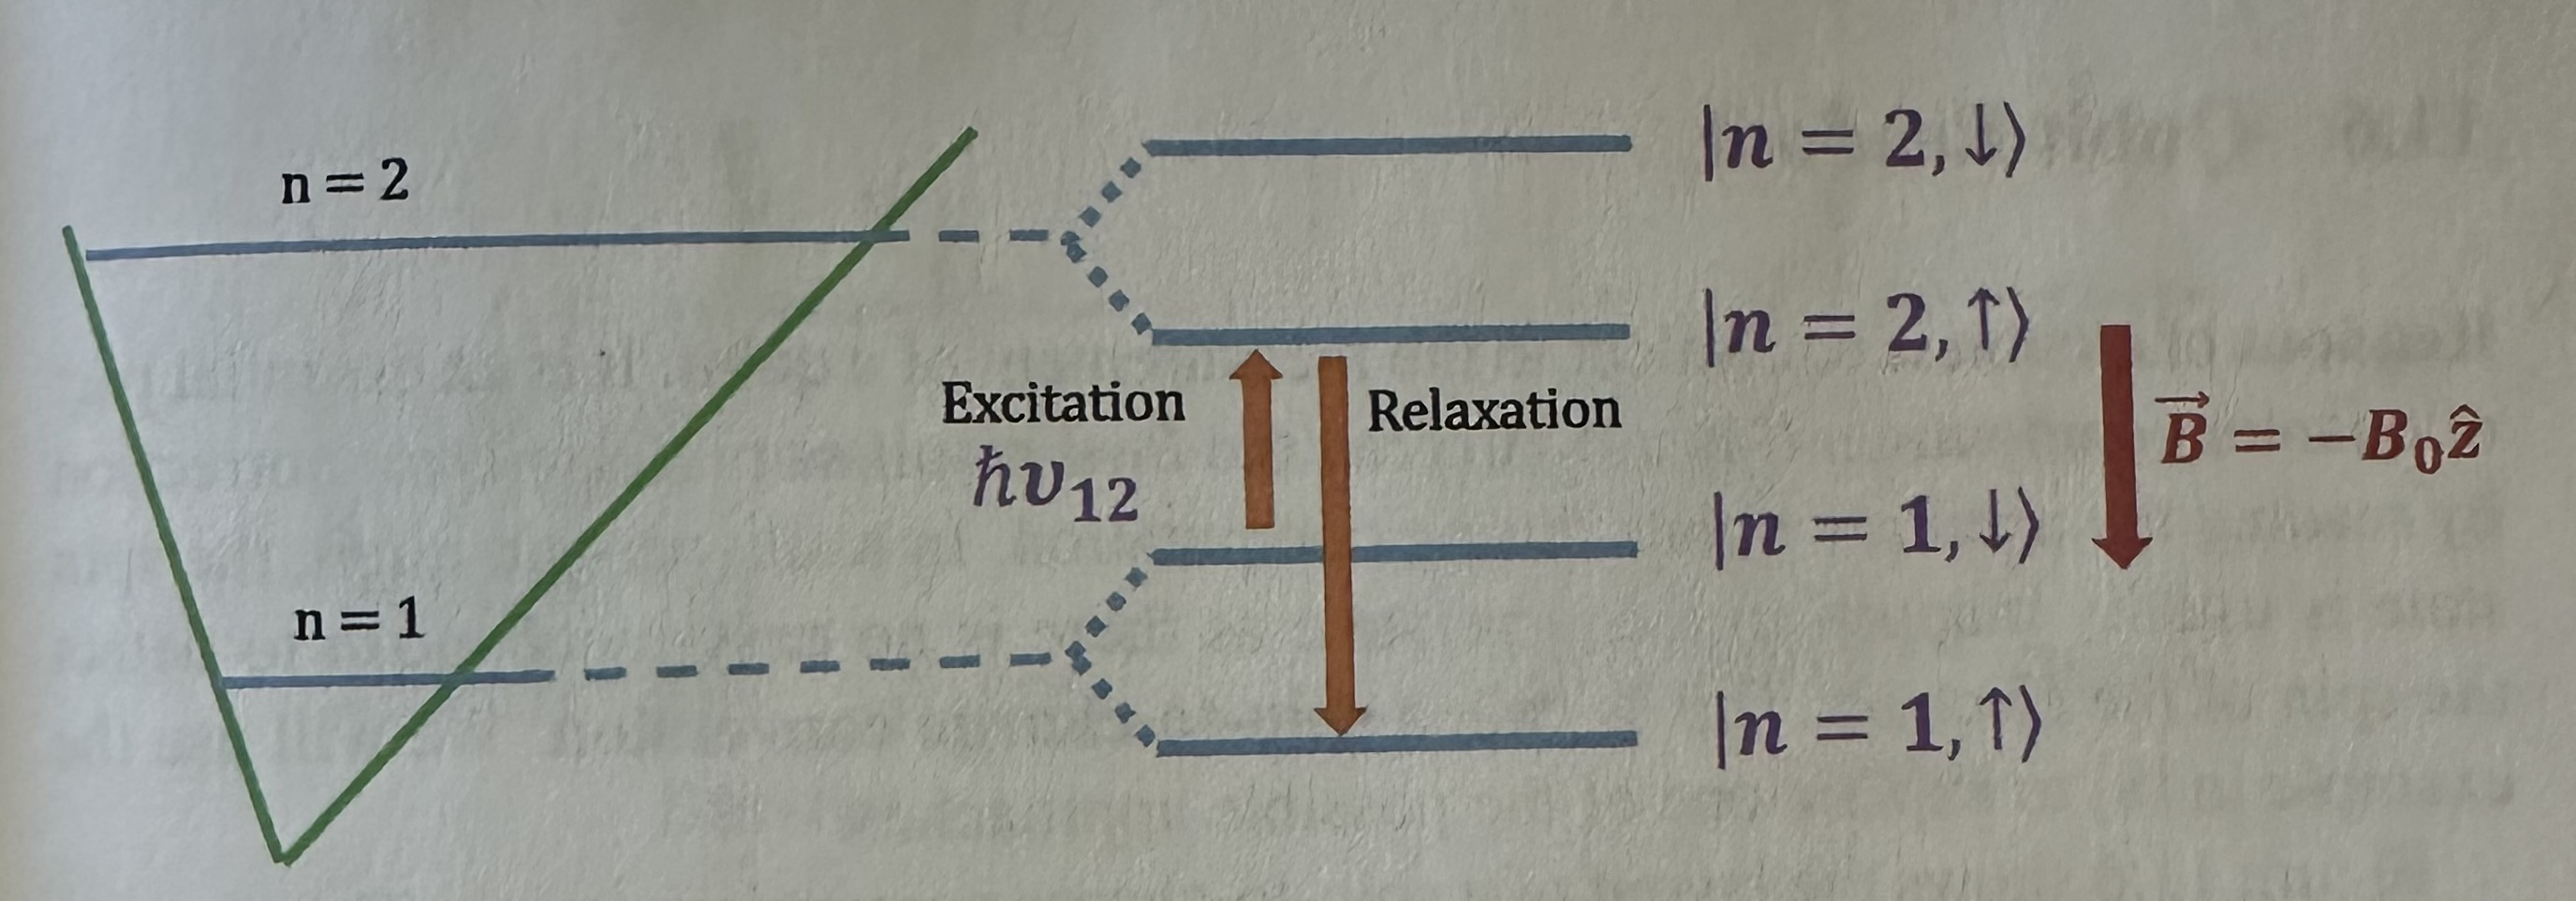
\includegraphics[scale=0.45]{Fig.11.5.jpeg}\\
\textbf{Fig. 11.5} Initialization scheme based on [9]. Left: Two orbital states formed due to an asymmertic
quantum well. Right: Both orbital states split into two levels due to Zeeman splitting\\\\\\
\bfit{\large 11.5.3 Initialization Through Higher Orbital State}\\\\
In [9], an initialization scheme through the interaction between two orbital states
is used. The scheme is shown in Fig. 11.5. Due to the confinement of the potential well,
there are multiple levels (just like the orbital levels of an electron in an atom). These energy
levels are \textit{not} due to the external magnetic fields. We will only discuss and use the lowest two
levels, i.e., $n=1$ and $n=2$. Note that in the previous discussion, we have been ignoring $n=2$. 
The qubit is encoded using the spin of the electron at $n=1$. Therefore, $\ket{0}$ is $\ket{\uparrow}$ at 
$n=1$ and $\ket{1}$ is $\ket{\downarrow}$ at $n=1$. We label them as $\ket{0}=\ket{n=1,\uparrow}$ and
$\ket{1}=\ket{n=1,\downarrow}$. We will similary label the splitting in $n=2$.

Note that $n=2$ is \textit{not} a part of the Hilbert space or the computing space. However, we will used n=2 states to help us
perfotmm initialization.

During initialization, we will apply a microwave pulse with an energy equal to
the energy difference between $\ket{n=1,\downarrow}$ and $\ket{n=2,\uparrow}$, which is $\hbar \nu_{12}$.
Note that equation in the chapter-end problem. If the qubit is $\ket{0}
=\ket{n=1,\uparrow}$, then the microwave energy is not enough to bring it to 
second orbital. Note that only a quantum of energy can be absorbed (i.e.,$\hbar \nu_{12}$).
So the qubit will stay at its ground state. However, if the qubit is in its excited state, $\ket{1}=\ket{n=1,\downarrow}$,
it will absorb one proton and become $\ket{n=2,\uparrow}$. Note that the spin direction is also flipped 
during the transition. This is possible because of the spin-orbit coupling which we will not
discuss and please take this for granted [9]. When it is at $n=2$, it decays rapidly to $n=1$ because of the
short lifetime (about 80 $ns$). The lifetime is much shorter thatn spin-relaxation (i.e., $T_1$ for relaxing
$\ket{n=1,\downarrow}$ to $\ket{n=1,\uparrow}$) which is $>1 ms$. Therefore, we can realize very rapid initialization.
For this scheme, we may say that we use an external microwave pulse to achieve spin flipping. Although
it is brought to a higher energy level ($n=2$), it will then relax naturally very fast to $n=1$.\\\\\\
\textbf{\large 11.6 Qubit Readout}\\\\
\textbf{Readout} of a qubit is equivalent to the measurement of a qubit. It is an essential part of
quantum computing. It is used to read the final result or perform error correction by reading the ancillary qubits
during computation.



\end{document}